\section{Introduction}
\label{sec:intro}
The problem of equivalence checking between a functional specification and an
implementation written in a low level imperative language such as C
has been of major research interest
and has several important applications such as (a) program verification, where
the equivalence checker is used to verify that the C implementation
behaves according to the specification and (b) translation validation, where
the equivalence checker attempts to generate a proof of equivalence across
the transformations (and translations) performed by an optimizing compiler
and more.

The verification of a C implementation against its manually written
functional specification through manually-coded refinement proofs has been
performed extensively in the seL4 microkernel \cite{seL4}.
Frameworks for program equivalence proofs have been developed in interactive
theorem provers like Coq \cite{programEquivalenceInCoq} where correlations and invariants
are manually identified during proof codification.
On the other hand, programming languages like Dafny \cite{dafny} offer automated program
reasoning for imperative languages with abstract data types such as sets and arrays.
Such languages perform automatic compile-time checks for manually-specified
correctness predicates through SMT solvers.
Additionally, there exists significant prior work on translation validation
\cite{tvi,tristan_tv_eqsat11,stepp_eqsat_llvm11,eqsat,pec,zuck03,zuck05,heffter05,covac,c_to_verilog,kanade09,lopes16,tvoc_cav05,ddec,semalign,oopsla20,tv_oskernel,namjoshi13}
across low level programming languages such as C and assembly\footnote{XXX:llvm ir also?}.
In most of these applications, soundness in critial,
i.e., if the equivalence checker determines the programs to be equivalent, then the programs are indeed equivalent
and evidently has equivalent observable behaviour. On the other hand, a sound equivalence checker may be incomplete
and fail to prove equivalence of a program pair, even if they were equivalent.

We present \toolName{}, a {\em sound} algorithm to automatically (push-button) search
for a proof of equivalence between a functional specification and its
optimized C implementations. We will demonstrate how \toolName{} is capable of
proving equivalence of multiple equivalent C implementations with vastly
different (a) data layouts (e.g. array, linked list representations of a {\em list})
and (b) algorithmic strategies (e.g. alternate algorithms, optimizations) against
a {\em single} functional specification.
This opens the possibility of regression verification \cite{strichman_regressverify,felsing14},
where \toolName{} can be used to automate verification across
software updates that change memory layouts for data structures.

\subsection{A Motivating Example}
\label{sec:motivatingexample}
We restrict our attention to programs that construct, read, and write
to recursive data structures. In languages like C, pointer and array based
implementations of these data-structures are prone to safety and liveness bugs.
Similar recursive data structures are also available in safer functional languages like Haskell,
where algebraic data types (ADTs) \cite{hope} ensure several safety properties.
We define a minimal functional language, called \SpecL{}, that enables the safe
and succinct specification of programs manipulating and traversing recursive data structures.
\SpecL{} is equipped with ADTs as well as boolean (\type{bool}) and fixed-size bitvector (\type{i<N>}) types.

We motivate our approach by considering example \SpecL{} and C programs.
We list the major hurdles of our approach and give an informal discussion on our proposed solutions.
We finish by stating our primary contributions in \cref{sec:contribs}.

\begin{figure}
\begin{tabular}{@{}c@{}c@{}}
\begin{subfigure}[b]{\textwidth}
\begin{center}
\begin{allLangEnvFoot}
~{\scriptsize \textcolor{mygray}{A0:}}~ type List = LNil | LCons (val:i32, tail:List).
~{\scriptsize \textcolor{mygray}{A1:}}~
~{\scriptsize \textcolor{mygray}{A2:}}~ fn mk_list_impl (n:i32) (i:i32) (l:List) : List =
~{\scriptsize \textcolor{mygray}{A3:}}~    if ${\tt i \geq_u n}$ then l
~{\scriptsize \textcolor{mygray}{A4:}}~             else make_list_impl(n, i+${\tt 1_{i32}}$, LCons(i, l)).
~{\scriptsize \textcolor{mygray}{A5:}}~
~{\scriptsize \textcolor{mygray}{A6:}}~ fn mk_list (n:i32) : List = mk_list_impl(n, ${\tt 0_{i32}}$, LNil).
\end{allLangEnvFoot}
\end{center}
\caption{\label{fig:llAllocSpec}Spec program}
\end{subfigure}%
\\
\begin{subfigure}[b]{\textwidth}
\begin{center}
\begin{allLangEnvFoot}
~{\scriptsize \textcolor{mygray}{B0: }}~ typedef struct lnode {
~{\scriptsize \textcolor{mygray}{B1: }}~   unsigned val; struct lnode* next;
~{\scriptsize \textcolor{mygray}{B2: }}~ } lnode;
~{\scriptsize \textcolor{mygray}{B3: }}~ 
~{\scriptsize \textcolor{mygray}{B4: }}~ lnode* mk_list(unsigned n) {
~{\scriptsize \textcolor{mygray}{B5: }}~   lnode* l = NULL;
~{\scriptsize \textcolor{mygray}{B6: }}~   for (unsigned i = 0; i < n; ++i) {
~{\scriptsize \textcolor{mygray}{B7: }}~     lnode* p = malloc(sizeof lnode);
~{\scriptsize \textcolor{mygray}{B8: }}~     p$\rightarrow$val = i; p$\rightarrow$next = l; l = p;
~{\scriptsize \textcolor{mygray}{B9: }}~   }
~{\scriptsize \textcolor{mygray}{B10:}}~   return l;
~{\scriptsize \textcolor{mygray}{B11:}}~ }
\end{allLangEnvFoot}
\end{center}
\caption{\label{fig:llAllocC}C program with {\tt malloc()}}
\end{subfigure}%
\\
\end{tabular}
\caption{\label{fig:llAllocSpecAndC}Spec and C programs each constructing a Linked List.}
\end{figure}


\Cref{fig:llAllocSpec,fig:llAllocC} show the construction of lists in \SpecL{} and C respectively.
The \type{List} ADT in the \SpecL{} program is defined at line \apc{0} in \cref{fig:llAllocSpec}.
An empty \type{List} is represented by the constructor \cons{LNil}, where as a non-empty list uses
the \cons{LCons} constructor to combine its first value ({\tt val}\ctype{i32}) and
the remaining list ({\tt tail}\ctype{List}).
The inputs to a \SpecL{} procedure are its well-typed arguments, which may include recursive data structure (i.e. ADT) values.
The inputs to a C procedure are its explicit arguments and the implicit state of program memory at procedure entry.
Similarly, the output of a C procedure consists of its explicit return value and the state of program memory at procedure exit.

The \SpecL{} procedure {\tt mk\_list} (defined at line \apc{6} in \cref{fig:llAllocSpec}), takes
a bitvector of size {\tt 32} ({\tt n}\ctype{i32}).
It returns a \type{List} value representing a linked list containing
the values {\tt (n-1)}, {\tt (n-2)}, ..., {\tt 1}, {\tt 0} starting from the head (the first value).
On the other hand, the C procedure {\tt mk\_list} (defined at line \bpc{3} in \Cref{fig:llAllocC})
constructs a {\em pointer based} linked list identical to the \SpecL{} procedure.
Unlike \SpecL{}, the construction of the linked list in C requires explicit allocation of memory through calls to {\tt malloc}
as well as, writes to the memory.
We are interested in showing that the \SpecL{} and C {\tt mk\_list} procedures are `equivalent'
i.e., given equal {\tt n} inputs, they both construct linked lists that are `equal'.

\begin{figure}[H]
\begin{tabular}{cc}
\begin{subfigure}[b]{0.37\textwidth}
\begin{center}
\begin{allLangEnvFoot}
~{\scriptsize \textcolor{mygray}{S0:}}~ List mk_list (i32 n) {
~{\scriptsize \textcolor{mygray}{S1:}}~   List l $\coloneqq$ LNil;
~{\scriptsize \textcolor{mygray}{S2:}}~   i32  i $\coloneqq$ ${\tt 0_{i32}}$;
~{\scriptsize \textcolor{mygray}{S3:}}~   while ${\tt \neg (i \geq_{u} n)}$:
~{\scriptsize \textcolor{mygray}{S4:}}~     l $\coloneqq$ LCons(i, l);
~{\scriptsize \textcolor{mygray}{S5:}}~     i $\coloneqq$ i + ${\tt 1_{i32}}$;
~{\scriptsize \textcolor{mygray}{S6:}}~   return l;
~{\scriptsize \textcolor{mygray}{SE:}}~ }
\end{allLangEnvFoot}
\vspace{35px}
\end{center}
\caption{\label{fig:llAllocSpecIR}(Abstracted) Spec IR}
\end{subfigure}%
&
\begin{subfigure}[b]{0.63\textwidth}
\begin{center}
\begin{allLangEnvFoot}
~{\scriptsize \textcolor{mygray}{C0:}}~ i32 mk_list (i32 n) {
~{\scriptsize \textcolor{mygray}{C1:}}~   i32 l $\coloneqq$ ${\tt 0_{i32}}$;
~{\scriptsize \textcolor{mygray}{C2:}}~   i32 i $\coloneqq$ ${\tt 0_{i32}}$;
~{\scriptsize \textcolor{mygray}{C3:}}~   while ${\tt i <_{u} n}$:
~{\scriptsize \textcolor{mygray}{C4:}}~     i32 p $\coloneqq$ malloc$_{\tt C4}$(sizeof(lnode));
~{\scriptsize \textcolor{mygray}{C5:}}~     $\mem{}$ $\coloneqq$ $\mem{}$[p+offsetof(lnode,val)$\leftarrow$i]$_\type{i32}$;
~{\scriptsize \textcolor{mygray}{C6:}}~     $\mem{}$ $\coloneqq$ $\mem{}$[p+offsetof(lnode,next)$\leftarrow$l]$_\type{i32}$;
~{\scriptsize \textcolor{mygray}{C7:}}~     l $\coloneqq$ p;
~{\scriptsize \textcolor{mygray}{C8:}}~     i $\coloneqq$ i + ${\tt 1_{i32}}$;
~{\scriptsize \textcolor{mygray}{C9:}}~   return l;
~{\scriptsize \textcolor{mygray}{CE:}}~ }
\end{allLangEnvFoot}
\end{center}
\caption{\label{fig:llAllocCIR}(Abstracted) C IR}
\end{subfigure}%
\\
\end{tabular}
\caption{\label{fig:llAllocSpecIRAndCIR}IRs for the \SpecL{} and C Programs in \cref{fig:llAllocSpec,fig:llAllocC} respectively.}
\end{figure}


For ease of comparison, we first convert both {\tt mk\_list} procedures to a common logical encoding, and call this the
intermediate representation (IR for short).
\Cref{fig:llAllocSpecIR,fig:llAllocCIR} show the intermediate representations of the \SpecL{} and C {\tt mk\_list}
procedures in \cref{fig:llAllocSpec,fig:llAllocC} respectively.
For the \SpecL{} procedure, the tail-recursive function {\tt mk\_list\_impl} is converted to a loop
and inlined in the top-level function {\tt mk\_list} in the IR.
For the C procedure in \cref{fig:llAllocC}, the memory state is made explicit (represented by the variable \mem{}),
and the size and memory layout (i.e. {\tt sizeof, offsetof}) of each type is concretized in the IR.
For example, the \type{unsigned} C type is encoded as the \type{i32} bitvector type.

Hence, we are interested in showing that the \SpecL{} and C IRs are `equivalent' i.e.,
given equal {\tt n} inputs, they both construct equal linked lists.
Since the argument {\tt n} to both procedures have identical types (i.e. \type{i32}),
their equality is quite trivially expressible i.e., $\sv{n} = \cv{n}$
\footnote{We use $S$ and $C$ subscripts to refer to variables in the \SpecL{} and C procedures respectively.}.
The \SpecL{} procedure uses the ADT \type{List} to represent a linked list.
However, the C procedure represents its returned linked list using a collection of \type{lnode} objects linked through
their \field{next} fields, and simply returns a value of type \type{i32} (\type{lnode*} in the original C program)
pointing to the first \type{lnode} in the list (or the null value representing an empty list).
To express equality between these two values (of types \type{List} and \type{i32}) representing linked lists, we
would like to `adapt' one of the values to a value matching the type of the other value.
We choose to lift the C linked list (represented by the \type{i32} value and the C memory state) to a \type{List} value
using an operator called a {\em lifting constructor}.
Let us call this lifting constructor \lift{list}{}{lnode} and the expression
\lifted{list}{\mem{}}{lnode}{p\ctype{i32}} represents a \type{List} linked list
constructed from a C pointer $p$ (pointing to a \type{lnode} object) in the memory state \mem{}.
We will formally define \lift{list}{}{lnode} in \cref{sec:recrel}.
This allows us to express equality between the outputs of the \SpecL{} and C procedures as:
$\sv{ret} = \lifted{list}{\mem{}}{lnode}{\cv{ret}}$, where \sv{ret} and \cv{ret} represents the
values returned by the respective \SpecL{} and C procedures in \cref{fig:llAllocSpecIR,fig:llAllocCIR}.
To further emphasize the fact that we are comparing (a) a \SpecL{} ADT value with (b) a ADT value
lifted from C values using a lifting constructor, we use `\indEq{}' instead of `$=$'
and call it a \recursiveRelation{}:
$\sv{ret} \indEq{} \lifted{list}{\mem{}}{lnode}{\cv{ret}}$.

\begin{figure}
\begin{tabular}{@{}c@{}c@{}}
\begin{subfigure}[b]{0.5\textwidth}
\begin{center}
{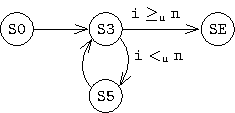
\includegraphics[scale=1.4]{chapters/figures/figMallocSpecCfg.pdf}}
\vspace{15pt}
\end{center}
\caption{\label{fig:llAllocSpecIRCFG}CFG of \SpecL{} program}
\end{subfigure}%
&
\begin{subfigure}[b]{0.5\textwidth}
\begin{center}
{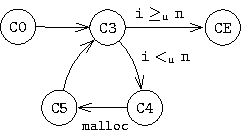
\includegraphics[scale=1.4]{chapters/figures/figMallocCCfg.pdf}}
\end{center}
\caption{\label{fig:llAllocCCFG}CFG of C program}
\end{subfigure}%
\\
\end{tabular}
\caption{\label{fig:mallocSpecCFGAndCCFG}CFG representation of Spec and C IRs shown in \cref{fig:llAllocSpecIR,fig:llAllocCIR} for the {\tt mk\_list} procedures in \cref{fig:llAllocSpec,fig:llAllocC} respectively.}
\end{figure}


Hence, we are interested in proving that given $\sv{n} = \cv{n}$ at the procedure entries,
$\sv{ret} \indEq{} \lifted{list}{\mem{}}{lnode}{\cv{ret}}$ holds at the exits of both procedures.
Before going into the proof method,
we first introduce an alternate representation of IR, called the Control-Flow Graph (CFG for short).
\Cref{fig:llAllocSpecIRCFG,fig:llAllocCCFG} show the CFG representation of the \SpecL{} and C IRs
in \cref{fig:llAllocSpecIR,fig:llAllocCIR} respectively.
Unlike the linear IR, CFG gives a graphical view of the control flow structures.
In essence, each node represents a PC location of its IR, and each edge represents (possibly conditional)
transition between PCs through instruction execution.
For brevity, we often represent a sequence of instructions with a single edge, e.g.,
in \cref{fig:llAllocCCFG}, the edge \cpath{5,3} represents the path \cpath{5,6,7,8,3}.

\begin{figure}[H]
\begin{tabular}{cc}
\begin{subfigure}[b]{1\textwidth}
\begin{center}
{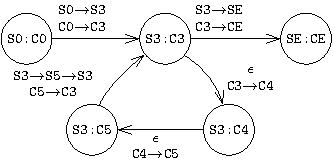
\includegraphics[scale=1.2]{chapters/figures/figMallocProductCfg.pdf}}
\end{center}
\end{subfigure}%
\end{tabular}
\caption{\label{fig:llAllocProductCFG}Product-CFG between \cref{fig:llAllocSpecIRCFG,fig:llAllocCCFG}}
\end{figure}


Due to the similarity of control flow (and loops) in the two procedures,
we choose {\em bisimulation} as our proof method.
Intuitively, a bisimulation relation encodes the execution of both procedures in lockstep
which ensures equal output lists.
Bisimulation can be represented as a {\em product program} \cite{covac}
and its CFG representation is called a {\em product}-CFG.
\Cref{fig:llAllocProductCFG} shows a product-CFG between the \SpecL{} and C procedures
in \cref{fig:llAllocSpecIRCFG,fig:llAllocCCFG} respectively.

\begin{table}[H]
\begin{center}
\caption{\label{tab:llproductInv}Node Invariants for Product-CFG in \cref{fig:llAllocProductCFG}}
\setlength{\belowcaptionskip}{-30pt}
\begin{footnotesize}
\begin{tabular}{|c|llll|}
\hline
\tt PC-Pair & \multicolumn{4}{c|} {\tt Invariants} \\
\hline
\hline
${\tt (S0:C0)}$ &
\multicolumn{4}{l|} {\Tstrut ${\tt { \circled{P}}\  n_{S}=n_{C}}$} \\
${\tt (S3:C3)}$ &
\Tstrut  ${\tt {\scriptsize \circled{I1}}\  n_{S}=n_{C}}$ & ${\tt {\scriptsize \circled{I2}}\  i_{S}=i_{C}}$ & ${\tt {\scriptsize \circled{I3}}\  i_{S} \leq_{u} n_{S}}$ & ${\tt {\scriptsize \circled{I4}}\  l_{S}\indEq{}Clist^{lnode}_{m}(l_{C})}$ \\
${\tt (S3:C4)\ (S3:C5)}$ &
\Tstrut  ${\tt {\scriptsize \circled{I5}}\  n_{S}=n_{C}}$ & ${\tt {\scriptsize \circled{I6}}\  i_{S}=i_{C}}$ & ${\tt {\scriptsize \circled{I7}}\  i_{S} <_{u} n_{S}}$ & ${\tt {\scriptsize \circled{I8}}\  l_{S}\indEq{}Clist^{lnode}_{m}(l_{C})}$ \\
${\tt (SE:CE)}$ &
\multicolumn{4}{l|} {\Tstrut  ${\tt {\circled{E}}\  ret_{S}\indEq{}Clist^{lnode}_{m}(ret_{C})}$} \\
\hline
\end{tabular}
\end{footnotesize}
\end{center}
\end{table}


At each node of the product-CFG, {\em invariants} relate the states of the \SpecL{} and C procedures respectively.
\Cref{tab:llproductInv} lists invariants for the product-CFG in \cref{fig:llAllocProductCFG}.
At the start node \scpc{0}{0} of the product-CFG, the precondition $Pre$ (labeled \circled{\small P})
ensures equality of input arguments \sv{n} and \cv{n} at the procedure entries.
Inductive invariants (labeled \circled{I}) need to be inferred at
each intermediate product-CFG node (e.g., \scpc{3}{3}) relating both programs' states.
For example, at node \scpc{3}{5}, \circled{\small I6} $\sv{i} = \cv{i}$ is an inductive invariant.
The inductive invariant \circled{\small I4} $\sv{l} \indEq{} \lifted{list}{\mem{}}{lnode}{\cv{l}}$
is another example of a \recursiveRelation{} and asserts equality between the intermediate \SpecL{} and C lists
at the loop heads.
Assuming that the precondition $Pre$ (\circled{\small P}) holds at the entry node \scpc{0}{0},
a bisimulation check involves checking that the inductive invariants hold too,
and consequently the postcondition $Post$ (\circled{\small E}) holds at the exit node \scpc{E}{E}.
Checking correctness of a bisimulation relation involves checking whether an invariant holds (along with many other things).
These checks result in proof queries which must be discharged by a theorem prover (i.e. a solver).

\subsection{Our Contributions}
\label{sec:contribs}
As previously summarized in \cref{sec:motivatingexample}, an algorithm to find a bisimulation based proof of equivalence
between a \SpecL{} and C procedure involves three major algorithms:
\circled{\footnotesize A1} An algorithm for construction of a product-CFG by correlating program executions
across the \SpecL{} and C programs respectively.
\circled{\footnotesize A2} An algorithm for identification of inductive invariants at intermediate correlated PCs.
\circled{\footnotesize A3} An algorithm for solving proof obligations generated by \circled{\footnotesize A1} and \circled{\footnotesize A2} algorithms.
Our major contributions are as follows:

\begin{itemize}
\item Proof Discharge Algorithm: Solving proof obligations (\circled{\footnotesize A3}) involving \recursiveRelations{}
(generated by \circled{\footnotesize A1} and \circled{\footnotesize A2}) is quite interesting and forms our primary contribution.
We describe a {\em sound} proof discharge algorithm capable of tackling proof obligations involving
\recursiveRelations{} using off-the-shelf SMT solvers. Our proof discharge algorithm is also capable of
reconstruction of counterexamples for the original proof query from models returned by the individual SMT queries.
These counterexamples are the backbone of counterexample-guided heuristics for \circled{\footnotesize A1} and \circled{\footnotesize A2} algorithms.
As part of our proof discharge algorithm,
we reformulate equality of ADT values (i.e. \recursiveRelations{}) as equivalence of their corresponding programs
and discharge these proof queries using a nested (albeit much simpler) bisimulation check.

\item Spec-to-C Automatic Equivalence Checker Tool: Our second contribution is \toolName{}, a {\em sound} equivalence checker tool
capable of proving equivalence between a \SpecL{} and a C program automatically.
\toolName{} either successfully finds a bisimulation relation implying equivalence or it provides a (sound but incomplete) unknown verdict.
\toolName{} is based on the Counter tool\cite{oopsla20} and uses modified versions of (a) counterexample-guided correlation algorithm for
incremental construction of a product-CFG (\circled{\footnotesize A1}) and (b) counterexample-guided invariant inference algorithm
for inference of inductive invariants at correlated PCs in the (partially constructed) product-CFG (\circled{\footnotesize A2}).
\toolName{} discharges required verification conditions (i.e. proof obligations) using our Proof Discharge Algorithm.
The counterexamples generated by the proof discharge algorithms help steer the search algorithms (\circled{\footnotesize A1}) and (for \circled{\footnotesize A2}).
\Cref{fig:diagram} gives an overview of the complete algorithm.
\end{itemize}

\begin{figure}
\begin{center}
{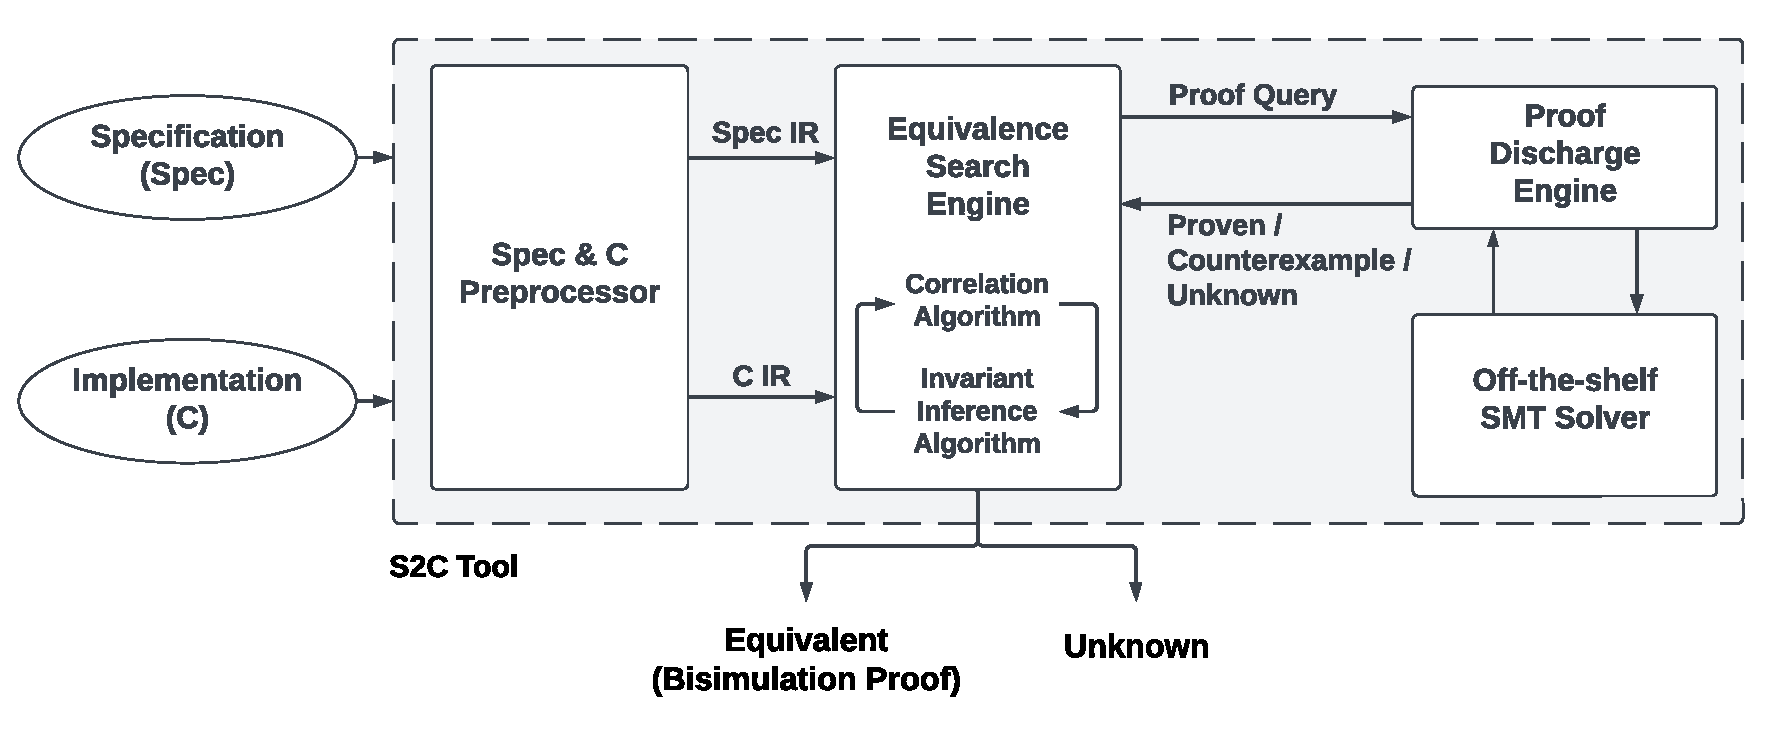
\includegraphics[scale=0.495]{chapters/figures/figDiagram.pdf}}
\end{center}
\caption{\label{fig:diagram}Overview of our equivalence checker algorithm \toolName{}.
The inputs to \toolName{} are the \SpecL{} and C programs.
\toolName{} either successfully finds a bisimulation proof implying equivalence or
soundly returns an unknown verdict.}
\end{figure}

\subsection{Outline of the Thesis}
\label{sec:outline}
\textbf{Chapter 1} of the thesis contains a general introduction to the research problem of verification C programs against a functional specification.
We take a C program and its analogue in a safe functional language, and contrast their differences.
We summarize our approach and finish with the major contributions.

\textbf{Chapter 2} begins with an introduction to a minimal function language `Spec' and an intermediate representation (IR).
The rest of this chapter provides a background on bisimulation relation and product program, as well as
introduce terminology used in the rest of the thesis.
We finish with a formal definition of equivalence.

\textbf{Chapter 3} starts with proof obligations and their properties.
The rest of the chapter gradually introduces our first contribution: A Proof Discharge Algorithm and related sub-procedures with the help
of two example programs introduced in the last two chapters. We also introduce a program representation of values, called `deconstruction program'.

\textbf{Chapter 4} contains a discussion on the two major components of our algorithm: (a) a counterexample-guided correlation algorithm
to search for a bisimulation relation and (b) a counterexample-guided invariant inference algorithm.
These two components along with our proof discharge algorithm allow automatic end-to-end equivalence checking.
We formalize handling of procedure calls, and finish with a dataflow formulation of a pointer analysis
used by our equivalence checker.

\textbf{Chapter 5} introduces a program graph representation of values, called `value graphs', similar to `deconstruction program'.
We motivate it by listing its advantages and give an algorithm to convert expressions to this representation.
This helps us simplify our proof discharge algorithm.

In \textbf{Chapter 6}, we introduce our automatic equivalence checker tool named \toolName{}, based on our proof discharge algorithm
and counterexample-guided search procedures.
\toolName{} is evaluated on a large variety of C programs involving lists, strings, trees and matrices.
This includes C programs taken from C library implementations as well as manually written programs. We show that our equivalence checker is able
to prove equivalence of a single specification with multiple C implementations, each varying in its data layout and algorithmic strategy.

Finally, \textbf{Chapter 7} discusses the limitations of our algorithm and draws comparison with some related work.
We note our key ideas and finish with potential improvements to our algorithm.